\documentclass[10pt, a4paper]{report}
\usepackage{amsmath}
\numberwithin{equation}{subsection}
\usepackage{graphicx}
\usepackage{titlesec}
\usepackage{appendix}
\usepackage[french]{babel}
\usepackage{xcolor,graphicx}
\usepackage[top=0.6in,bottom=0.6in,right=1in,left=1in]{geometry}
\usepackage{cite}
\usepackage{tocbibind}
\usepackage{siunitx}
\sisetup{output-exponent-marker=\ensuremath{\mathrm{e}}}
\usepackage{verbatim}
\usepackage{subcaption}
\usepackage{listings}
\begin{comment}
\usepackage{etoolbox}
\makeatletter
\patchcmd{\chapter}{\if@openright\cleardoublepage\else\clearpage\fi}{}{}{}
\makeatother
\end{comment}

\usepackage{ifpdf}
\ifpdf
\usepackage[pdftex]{hyperref}
\else
\usepackage{hyperref}
\fi


%\title{Stage M2 : Calcul du refroidissement moléculaire pour la formation des étoiles de population III}
%\author{Miville André}
%\date{Mars 2020}

\begin{document}





\begin{titlepage}
% \pagecolor{blue!10}
\begin{center}
	\begin{minipage}{2.5cm}
	\begin{center}
		
\includegraphics[width=3.0cm,height=1.7cm]{uga.png}
		
	\end{center}
\end{minipage}\hfill
\begin{minipage}{10cm}
	\begin{center}
	\textbf{ Université Grenoble Alpes}\\[0.1cm]
    \textbf{UFR Phitem}\\[0.1cm]
  %  \textbf{-Khouribga-}
% 		\textsc{\uppercase{Université Sultan Moulay Slimane}}
		
% 		\uppercase{éCOLE NATIONALE DES SCIENCES APPLIQUéES KHOURIBGA}
	\end{center}
\end{minipage}\hfill
\begin{minipage}{2.5cm}
	\begin{center}
		
\includegraphics[width=2.3cm,height=2.5cm]{cnrs.png}
	\end{center}

\end{minipage}
%\includegraphics[width=0.6\textwidth]{logo-isae-supaero}\\[1cm]
\textsc{\Large }\\[1.5cm]
{\large \bfseries Rapport de stage de Fin d'\uppercase{é}tudes}\\[0.5cm]
{\large En vue de l'obtention du diplôme}\\[1cm]

{\huge \bfseries \uppercase{Master de physique} \\[0.5cm] }
{\large \bfseries Filière : Astrophysique}
\textsc{\Large }\\[1cm]

% Title
\rule{\linewidth}{0.3mm} \\[0.4cm]
{ \huge \bfseries\color{blue!70!black} Calcul du refroidissement moléculaire pour la formation des étoiles de population III \\[0.4cm] }
\rule{\linewidth}{0.3mm} \\[1cm]
{\large \bfseries Organisme d'accueil : OSUG IPAG}\\[1cm]
% \includegraphics[width=0.3\textwidth]{logo-isae-supaero}\\[1cm]
% Author and supervisor
\noindent
\begin{minipage}{0.4\textwidth}
  \begin{flushleft} \large
    \emph{\color{orange!80!black}Réalisé par :}\\
    M.~\textsc{Miville} André\\
  \end{flushleft}
\end{minipage}%
\begin{minipage}{0.5\textwidth}
  \begin{flushright} \large
    \emph{\color{orange!80!black}Sous la direction de :} \\
    M.~\textsc{Faure} Alexandre (CNRS)\\
    M.~\textsc{Hilly-Blant} Pierre (UGA)\\
  \end{flushright}
\end{minipage}\\[1cm]

\color{blue!80!black}{\large \textit{Soutenu le 01 juillet 2019, Devant le jury : }}\\[0.5cm]

\color{black}
\centering
\begin{tabular}{lll}
\large Pr.~Meriem \textsc{Mandar} : & \large ENSA Khouribga & \large - Présidente \\[0.1cm]
\large Pr.~Mohamed \textsc{Amnai} : & \large ENSA Khouribga & \large - Encadrant \\[0.1cm]
\large Pr.~Mohammed \textsc{Nasri} : & \large ENSA Khouribga & \large - Encadrant
\end{tabular}

\vfill

% Bottom of the page
{\large \color{orange!80!black}{Année universitaire}\\ \color{blue!80!black}2019/2020}

\end{center}
\end{titlepage}





































%\maketitle
\renewcommand{\contentsname}{Sommaire}
\renewcommand{\bibname}{Références}



%\addcontentsline{toc}{chapter}{Quelques rappels de Relativité Générale} 
\tableofcontents


\chapter*{Remerciements}
\addcontentsline{toc}{chapter}{Remerciements} 
Je remercie expréssement mes deux maîtres de stage M. \textsc{Faure} Alexandre et M. \textsc{Hilly-Blant} Pierre pour l'encadrement du stage, leurs encouragements, leurs conseils ainsi que leur aide apportée à la réalisation de ce rapport.

Je remercie aussi M. \textsc{Henri} Gilles pour sa relecture de l'annexe concernant la relativité générale et sa disponibilité sans faille à répondre à mes nombreuses interrogations.

Finalement j'exprime ma gratitude envers mes parents qui m'ont légué des valeurs qui se complètent et qui expliquent en outre le succès relatif de mon parcours de vie et envers mon oncle qui m'a poussé à faire des études.
 

\chapter*{Introduction}
\addcontentsline{toc}{chapter}{Introduction} 
\addcontentsline{toc}{section}{Missions effectuées}
\addcontentsline{toc}{section}{Conventions utilisées}
La formation des premières étoiles, dites de population III, a lieu avant l'époque de reionisation, à un décalage vers le rouge cosmologique $\approx$20. Bien que les contraintes observationnelles directes sur la formation de ces premières étoiles soient inexistantes, des contraintes indirectes seront obtenues dans les 10 prochaines années. D'ailleurs, plusieurs interféromètres radio observant la raie de l'hydrogène atomique à 21 cm, décalée vers le rouge, ont d'ores et déjà commencé a accumulé des données, et de futurs instruments tels que SKA, l'E-ELT, ou le JWST, produiront des images du milieu intergalactique neutre et des galaxies à des redshifts $>$10.

Une question fondamentale pour la formation des premières étoiles est celle du refroidissement du gaz baryonique piégé dans les halos de matière noire. De l'efficacité de ce refroidissement dépendra la masse des premières étoiles, et ainsi la rétroaction sur l'évolution de la matière baryonique au cours de la naissance des premières structures. \begin{comment}D'après le modèle $\Lambda $CDM, la nucléosynthèse primordiale crée principalement des atomes d'hydrogène et d'Hélium. Avant les premières étoiles, les molécules régissant le refroidissement moléculaires sont alors simples. Dans mon stage nous nous sommes concentré sur H2. Les détails de la formation de H2, et notamment de ses formes ortho et para, sont donc essentiels.\end{comment}

Le stage se déroule en deux étapes. Il s'agit d'abord de simuler un univers homogène et isotrope en expansion avec un modèle $\Lambda$CDM jusqu'au décalage vers le rouge cosmologique d'effondrement gravitationnel. Ceci nous permet d'avoir des conditions initiales propres pour un second modèle avec effondrement qui calcule le refroidissement moléculaire pour la formation des étoiles POP III. Dans ce rapport seule la première partie sera traitée.

La simulation d'univers homogène et isotrope pour les conditions initiales sur la chimie n'est pas un travail inédit en soi, d'autres chercheurs ont déjà effectué des recherches similaires comme Gallli D. et al, Coppola CM. et al, Pineau des forêts G. et al. De nouvelles données de calcul quantique dernier cri de taux de collisions moléculaires par l'équipe de Lique F. et al. ont donné l'opportunité d'améliorer et de compléter les résultats existants. 

La problématique de notre sujet demande d'avoir une vue d'ensemble sur différentes spécialités en physique ($\Lambda CDM$, effondrement, chimie moléculaire, transfert radiatif). Notre petite équipe n'est pas experte dans tous les domaines. Notamment le modèle $\Lambda CDM$ où il a fallu se mettre à jour. Par conséquent une grosse partie du stage a concerné la compréhension dans les grandes lignes de ce modèle, afin de pouvoir l'utiliser en version simplifié et l'appliquer à notre objectif de calcul du refroidissement moléculaire.
%Par ailleurs l'augmentation continue de la puissance de calcul des processeurs permet l'implémentation de modèles toujours plus évolués.
%Mes maîtres de stage se sont saisi de l'occasion pour se lancer et découvrir cette problématique externe à leur expertise initiale. 




\section*{Missions effectuées}

Durant ces quatre mois de stage, j'ai été amené à réviser la relativité générale, le transfert de rayonnement, la mécanique quantique, la chimie moléculaire à me documenter sur le modèle $\Lambda$CDM, à redémontrer et fournir les formules utilisées dans les publications de références et de notre modèle, à programmer en C, Fortran, python, bash, à réaliser un intégrateur Runge Kutta, à interfacer des programmes entre eux, à produire des courbes/graphiques de résultats, à faire des présentations, à écrire un rapport de stage.

%\chapter*{Quelques rappels de Relativité Générale}


\section*{Conventions utilisées}

Dans ce rapport, on utilise :
\begin{itemize}
	\item[$-$] La convention de signe $(-++)$ en rapport à la classification des signes établi par Misner, Thorne, et Wheeler.
	\item[$-$] Les unités SI, pas d'unités naturelles.
	\item[$-$] La définition de la quadrivitesse suivante : $u^\mu = \frac{{\rm d}x^\mu}{{\rm d}\tau}$ avec $\tau$ le temps propre
	\item[$-$] $\rho$ peut être une densité massique ou énergétique (dépend du contexte).
\end{itemize}



\chapter{Préliminaire : l'Univers en expansion}
Un formulaire et rappel de Relativité Générale est disponible en annexe de ce rapport. 

\section{Le principe cosmologique et la métrique FLRW}
En Relativité Générale, l'équation d'Einstein permet de faire évoluer la forme de l'espace temps -associé à la métrique et au champ d'accélération gravifique- en fonction de la distribution d'énergie ou de masse sur cette espace temps. Problème, pour qu'une distribution d'énergie dans l'univers est un sens, il faut d'abord définir une forme d'univers sur lequel on place les masses. La condition initiale de la forme de l'univers pose alors un certain problème qu'on résoud grâce au principe cosmologique.

En termes simples, le principe cosmologique d'homogénéité et d'isotropie spatial est l'hypothèse selon laquelle il n'y a pas d'endroit ni de direction privilégié dans l'espace spatial. On place un observateur cosmique comobile en chacun des points de l'espace spatial et la métrique associée ne dépend pas du point spatial où l'on se situe car ils sont tous équivalents. Points spatiaux car l'univers n'est pas identique à lui même par translation dans le temps. Le temps relié à ces observateurs s'appelle le temps cosmique. Un espace spatial à courbure constante à un instant donné est un espace spatial homogène et isotrope.  La constatation expérimentale de l'expansion de l'univers permet de justifier l'apparition d'un facteur d'échelle dépendant du temps cosmique. La métrique de Friedmann–Lemaître–Robertson–Walker rend compte de ces hypotèses.

En coordonnées sphériques $(r, \theta, \phi)$ la métrique FLRW, se note :

\begin{equation}
\boxed{ c^2 {\rm d}\tau^2 = c^2 {\rm d}t^2 - a(t)^2 \left (\frac{{\rm d}r^2}{1 - k r^2} + r^2 ({\rm d}\theta^2 + \sin^2 \theta \; {\rm d} \phi^2) \right )}
\end{equation}

en  où :
* $a(t)$ est le rayon de l'univers;
* $k$ est le facteur de courbure. $k = \{-1,0,1\}$ pour un espace respectivement à courbure ouverte (correspondant à une géométrie hyperbolique), à courbure nulle (correspondant à l'espace euclidien) et à courbure fermée (correspondant à la surface d'une sphère de dimension 4) ;
* $t$ est le temps cosmique.

Les observations ne nous permettent pas encore de nous prononcer sur la valeur du facteur de courbure $k$ de notre univers mais elles suggèrent que la courbure actuelle de l'espace est plus ou moins nulle $ \kappa \approx 0 \pm [\num{1e-4}]$. Dans ces conditions prendre $k=0$ n'est pas déconseillé et permet de simplifier les raisonnements et les formules. Dans la suite de ce rapport nous nous restreindrons à $k=0$. 
\subsection{Distances physiques}
Prenons des coordonnées cartésiennes avec notre espace plat. Soit deux points au même instant $t_0$ séparé par une distance comobile $\Delta X$. Pour évaluer la distance physique séparant ces deux points, on peut faire propager un photon les reliant et multiplier le temps de parcours par la vitesse de la lumière pour avoir la-dite distance physique. On a donc un intervalle de genre lumière et on montre sans difficultés que \begin{equation}
\boxed{ L=\int\limits_0^{\Delta X} a(t)dx}
\end{equation}
avec \begin{equation}
\boxed{ t=t_0 + \int\limits_0^x a(t')dx'}
\end{equation}
De sorte qu'au premier ordre on a :
\begin{equation} \label{eq:foL}
\boxed{ L \approx a(t_0) * \Delta X}
\end{equation}
\subsection{Décalage vers le rouge cosmologique}
Le décalage vers le rouge $z$ est par définition : 
\begin{equation}
\boxed{1+z = \frac{\lambda_{\mathrm{obsv}}}{\lambda_{\mathrm{emit}}}}
\end{equation}

Le décalage vers le rouge cosmologique est le décalage dû à l'expansion de l'univers. En considérant que le nombre de noeuds d'un photon dans une cavité du vide de longeur L à l'instant $t_0$ est conservé au cours du temps, on montre en utilisant la formule approchée \ref{eq:foL} que :
\begin{equation} \label{eq:zC}
\boxed{1+z = \frac{a(t_{pr\acute esent})}{a(t_{\acute emission})}}
\end{equation}

En fait cette dernière équation est tout le temps vraie.

\section{\uppercase{é}quation d'Einstein avec la métrique FLRW}
On rappelle l'équation d'Einstein :
\begin{equation} \label{eq:EFE}
\boxed{R_{\mu \nu} \ - \ \frac{1}{2} \, g_{\mu \nu} \, R  \  =  \kappa T_{\mu \nu}}
\end{equation}
Que prendre alors pour le tenseur énergie-impulsion ?
\subsection{Le fluide parfait}
On modélise les formes d'énergies dans l'univers comme fesant partie d'un fluide parfait de densité énergétique $\rho$ au repos par rapport à un observateur cosmique exerçant une pression $P$. Son équation est : 

\begin{equation} \label{eq:FP}
\boxed{T_{\mu\nu} = (P + \rho) u_\mu u_\nu - P g_{\mu\nu}}
\end{equation}

\subsection{Les équations de Friedmann}
On égalisant des deux cotés de l'équation d'Einstein, on déduit après un long calcul les équations de Friedmann :

\begin{equation} \label{eq:F1}
\boxed{3 \left(\frac{H^2}{c^2} + \frac{K}{a^2 c^2} \right) = \frac{8 \pi G}{c^4} \rho}
\end{equation}
\begin{equation} \label{eq:F2}
\boxed{- 2 \frac{\dot H}{c^2} - 3 \frac{H^2}{c^2} - \frac{K}{a^2 c^2} =  \frac{8 \pi G}{c^4} P }
\end{equation}
On peut réexprimer la seconde équation grâce à la première en une forme plus pratique qui donne la dérivée de la densité énergétique :
\begin{equation} \label{eq:F3}
\boxed{\frac{{\rm d}\rho}{{\rm d}t} = - 3 H (P + \rho) }
\end{equation}
Si la pression est propotionnelle à la densité : $P= w \rho$ alors \ref{eq:F3} possède une solution analytique :
\begin{equation} \label{eq:F3S}
\boxed{\rho = Cste \times a^{-3(1+w)}}
\end{equation}
Si la densité est composé de deux espèces différentes comme par exemple la densité d'énergie de masse de la matière et celle du champ radiatif alors l'équation \ref{eq:F3} se découple en deux équations indépendantes : Si $\rho = \rho_m + \rho_r$ alors on a séparément $\frac{{\rm d}\rho_m}{{\rm d}t} = - 3 H (P_m + \rho_m) $ et $\frac{{\rm d}\rho_r}{{\rm d}t} = - 3 H (P_r + \rho_r)$.



\subsection{Densité critique}
La densité critique énergétique est la densité telle que l'expansion est nulle pour une courbure nulle ou négligeable. On comprend l'expression formelle de sa définition à partir de l'équation de Friedmann 1 : (voir eq: \ref{eq:F1})

\begin{equation} \label{eq:DEC}
\boxed{\rho_{\rm c} \equiv \frac{3 c^2 H^2 }{8 \pi G} }
\end{equation}

On exprime souvent la densité d'énergie d'un certain type par son rapport sans dimension avec la densité critique qu'on appelle paramêtre de densité :

\begin{equation} \label{eq:OD}
\boxed{\Omega \equiv \frac{\rho}{\rho_{\rm c}} }
\end{equation}

\subsection{Notre intégrateur et solutions classiques}
Un intégrateur qui résout l'expansion en fonction du temps a dû être développé. Nous montrons les résultats de notre intégrateur sur des cas d'écoles simples tel que l'Univers de De Sitter et l'Univers d'Einstein-De Sitter. Le temps cosmique normalisé est le temps sans dimension : $t' = H_0 \times t$. Pour distinguer les deux courbes, des points discrêts ont été tracés au lieu d'une ligne continue. L'intégrateur reproduit parfaitement les courbes attendues. Le temps nul correspond à actuellement et le facteur d'échelle y est pris à 1. L'intégrateur remonte dans le temps. On retrouve dans l'univers de poussière d'Einstein-De Sitter que l'univers survit deux tiers du temps de Hubble : $\frac{2}{3H_0}$ 

\begin{figure}[h]

\begin{subfigure}{0.5\textwidth}
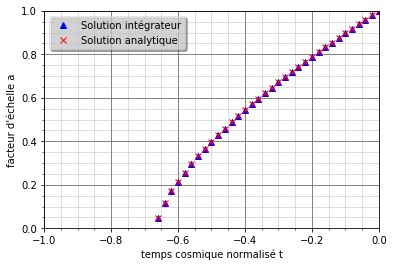
\includegraphics[width=8.0cm,height=6cm]{EDSf.png}
\caption{Univers Einstein-De Sitter}
\label{fig:UEDS}
\end{subfigure}
\begin{subfigure}{0.5\textwidth}
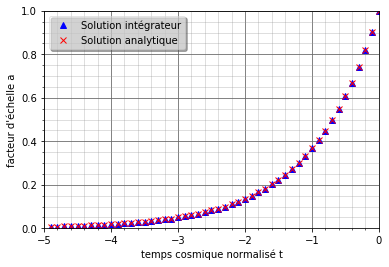
\includegraphics[width=8.0cm,height=6cm]{DSf.png}
\caption{Univers De Sitter}
\label{fig:UDS}
\end{subfigure}

\caption{Comparaison des solutions analytiques et intégrateur}
\label{fig:UISC}
\end{figure}



\chapter{Notre modèle simplifié inspiré du modèle $\Lambda$CDM}
$\Lambda$ est la constante cosmologique et CDM est l'acronyme de Cold Dark Matter. C'est avant tout une théorie à paramètres. La fameuse matière noire n'est toujours pas identifiée. La valeur de la constante cosmologique est le résultat d'un ajustement. Néanmoins cette théorie permet d'expliquer avec une grande validité diverses constatations astrophysiques. Nous n'avons pas besoin d'en comprendre tous les détails pour poursuivre l'objectif de ce stage.

\section{Valeurs des paramètres par la mission Planck 2018}
Ci-dessous les valeurs utilisées dans notre modèle. Elles sont calculées ou prises dans le tableau 2 colonne "TT,TE,EE+lowE+lensing" du papier "Planck 2018 results. VI. Cosmological parameters".

\begin{center}
\begin{tabular}{ m{5cm} m{5cm} } 
 \hline
 Paramètre & Valeur numérique\\ 
 \hline
$\Omega_m$ & 0.3153\\ 
$\Omega_{dm}$ & cell5\\ 
$\Omega_b$ & cell5\\ 
$\Omega_r$ & cell5\\
$\Omega_K$ & 0.000\\
$\Omega_\Lambda$ & 0.6847\\ 
$\eta_{10}$ & cell5\\ 
$z_{eq}$ & 3402\\
$T_0$ & cell5\\ 
$H_0 [km s^{-1} Mpc^{-1}]$ & 67.36\\ 
 \hline
\end{tabular}
\end{center}

\section{La constante cosmologique et l'énergie noire}
L'équation d'einstein avec constante cosmologique s'écrit:
\begin{equation} \label{eq:EFEL}
\boxed{R_{\mu \nu} \ - \ \frac{1}{2} \, g_{\mu \nu} \, R  \ + \ \Lambda \ g_{\mu \nu} \ =  \kappa T_{\mu \nu}}
\end{equation}
On peut cependant interprêter la constante cosmologique comme un fluide parfait de densité d'énergie positive constante qu'on appelle énergie noire et de pression négative avec pour équation d'état :
\begin{equation} \label{eq:EEL}
\boxed{P_\Lambda=-1 \times \rho_\Lambda}
\end{equation}
La méthode est de poser un nouveau tenseur énergie-impulsion qui inclut en son sein la constante cosmologique grâce à un changement de variable. On obtient finalement que la densité volumique d'énergie noire vaut :
\begin{equation} \label{eq:DEL}
\boxed{\rho_{\Lambda}  =  \frac{c^4 \Lambda}{8\pi G}}
\end{equation}

\section{La matière noire et baryonique froide}
La matière noire est nécessaire pour expliquer diverses observations astrophysiques. Elle est supposée interagir uniquement par gravité. On suppute aussi qu'elle est froide de sorte que seule son énergie de masse compte pour le calcul de la densité d'énergie. 
Dans notre stage, nous nous intéressons à une période de l'univers où la température de la matière baryonique est inférieure à 10 000K. Cette température est considéré comme froide en comparaison à l'énergie de masse. Donc pareillement à la température de la matière noire, la température baryonique n'intervient pas dans le calcul de la densité d'énergie, seule son énergie de masse compte. Cela revient à considérer que la matière est immobile et exerce une pression nulle.
Son équation d'état est donc :
\begin{equation} \label{eq:EEM}
\boxed{P_m=0 \times \rho_m c^2}
\end{equation}
avec $\rho_m$ la densité de masse de la matière noire et baryonique
D'après \ref{eq:F3S}, on obtient que

\begin{equation} \label{eq:DEM}
\boxed{\rho_{\rm m}(t) = \rho_{\rm m}(t_0) \left(\frac{a(t_0)}{a(t)}\right)^3}
\end{equation}

Nous pouvons aussi retrouver simplement cette équation par un raisonnement sur la densité particulaire qui varie telle que 
\begin{equation} \label{eq:NP}
\boxed{n(t) = n(t_0) \left(\frac{a(t_0)}{a(t)}\right)^3}
\end{equation}

\section{Le champ de rayonnement électromagnétique et les neutrinos}
La découverte du fond diffus cosmologique a eu impact retantissant en cosmologie. Grâce à lui nous pouvons savoir notre vitesse par rapport à un observateur cosmique, définissant en quelque sorte un référentiel privilégié, fait rare en RG ! 
\subsection{La température de radiation}
Le fond diffus est dû à un rayonnement primordial qui s'est refroidi avec l'expansion et dont la distribution en fréquence se modélise comme un corps noir presque parfait de température T dont la distribution est donnée par la loi de planck. En plaçant des photons dans une cavité du vide de longueur L, on montre fortunément que le refroidissement adiabatique dû à l'expansion d'un corps noir est un corps noir de température amoindrie, de sorte que $T_r$ évolue en $T_{r0} (1+z)$:
\begin{equation} \label{eq:TRRA}
\boxed{T_r(t) = T_r(t_0) \frac{a(t_0)}{a(t)}}
\end{equation}
\subsection{\uppercase{é}quation d'état}
Par le même raisonnement on montre que la densité d'énergie radiative évolue en $\rho_{r0} (1+z)^4$ :
\begin{equation} \label{eq:DER}
\boxed{\rho_r(t) = \rho_r(t_0)  \left({\frac{a(t_0)}{a(t)}}\right)^4}
\end{equation}

Avec la distribution de planck on trouve le tenseur énergie impulsion du champ radiatif et le résultat bien connnu que la pression radiative vaut le tiers de l'énergie radiative (pour un corps noir) :
\begin{equation} \label{eq:EER}
\boxed{P_r = \frac{1}{3} \times \rho_r}
\end{equation}
Grâce à l'équation d'état on peut utiliser \ref{eq:F3S} pour retrouver \ref{eq:DER} 

\subsection{Neutrinos}

%\subsection{Refroidissement adiabatique des photons dû à l'expansion}
%\subsection{Refroidissement adiabatique des neutrinos dû à l'expansion}

\section{Intégrateur et solution simplifiée de l'expansion}
Au vu de ce qui a été dit depuis le début, l'équation de Friedmann 1 (\ref{eq:F1}) s'écrit pour nos conditions :

\begin{equation} \label{eq:ELCDM}
\boxed{a' = \sqrt{\Omega_{\Lambda}*a^2+\Omega_{m0}/a+\Omega_{ro}/a^2}}
\end{equation}
avec $a'$ la dérivée par rapport au temps cosmique normalisé. Le temps cosmique normalisé est le temps sans dimension : $t' = H_0 \times t$.  Le temps nul correspond à actuellement et le facteur d'échelle y est pris à 1. L'intégrateur remonte dans le temps. L'Univers survit une portion d'environ 0.95 du temps de Hubble. 

\begin{figure}[h]
\centering
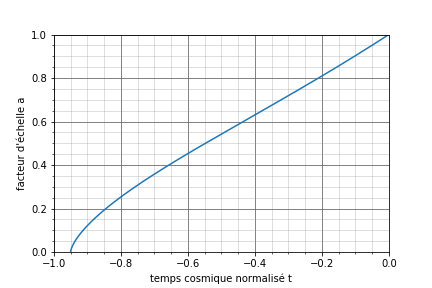
\includegraphics[width=12.0cm,height=9cm]{LCDMf.png}
\caption{Univers $\Lambda$CDM simplifié}
\label{fig:ULCDM}
\end{figure}
 

\chapter{L'époque de réionisation}
\section{La température baryonique}
\subsection{Refroidissement adiabatique dû à l'expansion}
\section{\uppercase{é}changes d'énergie entre photons et électrons}
\subsection{Nombre de photons par baryons}

\subsection{Processus Compton}
C'est le processus de diffusion d'un photon sur un électron libre, il a une importance capitale en cosmologie à cause de sa grande section efficace. La diffusion d'un photon sur un proton a quant à lui une section efficace environ mille fois plus faible et peut donc être négligé. On rappelle les résultats principaux. Dans le référentiel de l'électron au repos, le photon de longeur d'onde $\lambda$ arrivant sur l'électron défini une direction privilégiée. Dans cette configuration, l'électron ne peut que gagner de l'énergie. On note $\theta$ l'angle avec lequel sera éjecté l'électron par rapport à cette direction, la direction incidente du photon. Comme on néglige les effets de spin de l'électron et du photon, on peut ramener cette collision à un problème 2d.
La variation de longeur d'onde vaut :
\begin{equation} \label{eq:VLO}
\boxed{\Delta\lambda=\frac{h}{m_e c}(1 - \cos \theta)}
\end{equation}

 Le premier ordre non trivial de l'électrodynamique quantique nous dit que la section efficace différentielle non polarisée vaut :
\begin{equation} \label{eq:QED}
\boxed{\frac{d\sigma}{d\Omega} = \frac{1}{2} r_e^2 \left(\frac{\lambda}{\lambda'}\right)^{2} \left[\frac{\lambda}{\lambda'} + \frac{\lambda'}{\lambda} - \sin^2(\theta)\right]}
\end{equation}

\subsection{Processus Compton Inverse}
Si l'électron n'est pas au repos, on peut toujours faire un changement de référentiel pour avoir l'électron au repos et appliquer la théorie du processus Compton, puis faire un changement de référentiel inverse pour revenir au référentiel initial où l'électron se meut. L'électron ou le photon peut alors avoir gagné ou perdu de l'énergie.
\subsection{Diffusion Thompson}
La diffusion Thompson est la limite basse énergie de la diffusion Compton. Dans cette approximation, le photon accélère une particule chargée qui rayonne. Ce rayonnement est alors interprété comme étant la diffusion du photon sur la particule chargée. Le photon ne perd pas d'énergie mais la particule reçoit un flux net d'impulsion qu'on convertit en énergie gagnée. On l'a soustrait ensuite à l'énergie des photons. Malheureusement la distribution en fréquence des photons ne suit plus celle d'un corps noir. Mais un argument simple sur le nombre de photons par baryons dit que le pourcentage de photons qui aura interagi sera très faible et ne modifiera pas sensiblement la statistique. À première vue, 
Pour calculer les échanges d'énergies au premier ordre entre les températures baryoniques et de rayonnement une approche similaire est utilisée. Peebles a montré qu'un électron se déplaçant à la vitesse $v<<c$ avec une direction $\theta $ par rapport à la direction d'un photon voit une température radiative apparente de 

  

 
\subsection{Fraction d'ionisation $x_e$}
\section{Paramètre $z_{eq}$}
Il correspond au décalage vers le rouge cosmologique où la densité énergétique de rayonnement est égale à celle de la matière. \uppercase{é}tant donné que le terme compensateur Compton est très important, il force la température baryonique à être environ égale à la température de rayonnement : $T_b \approx T_r$ de sorte que l'on utilise cette condition intiale dans notre programme.

\chapter{Refroidissement moléculaire}
%\section{\uppercase{é}léments de transfert de rayonnement}
\section{Le programme RADEX}
\section{La molécule H2}
\subsection{Forme ortho et para}
\subsection{\uppercase{é}quation d'évolution des niveaux}
\subsection{Rapport ortho para}

\addcontentsline{toc}{chapter}{Conclusion} 
\chapter*{Conclusion}


\appendix
\begin{comment}
\chapter{Formules utiles et rappels de Relativité Générale}
\section{Généralités}
La relativité générale est une théorie décrivant la forme de l'espace temps par la théorie mathématique des variétés courbes. Le principe d'équivalence d'Einstein est la base physique de la théorie. Il dit que l'observateur en chute libre, c'est à dire celui accéléré par le champ gravifique est localement inertiel, i.e. la relativité restreinte s'applique. Lorsqu'on tente d'appliquer ce principe, on s'aperçoit que cela n'est pas possible dans un espace-temps plat mais possible dans une autre théorie comme celle des variétés courbes. Dans ce formalisme, on munie une variété différentielle par une connexion affine qui connecte les espaces tangents. En relativité générale on utilise la connexion de Lévi-Civita. La "distance" utilisée est l'intervalle d'espace temps qui mesure physiquement le temps propre pour l'observateur comobile à la ligne d'univers considérée. 

\section{Coordonnées généralisés}
\subsection{base naturelle}


\section{Connexion}
\subsection{Généralités}
Sur toute variété, on peut définir une infinité de connexions affines. Le choix d'une connexion affine est équivalent à définir une façon de dériver les champs de vecteurs. Un choix de connexion affine est aussi équivalent à une notion de transport parallèle, c'est-à-dire à un moyen de transporter les vecteurs le long de courbes de la variété. Les principaux invariants d'une connexion affine sont sa courbure et sa torsion.


\subsection{Coefficients $\&$ symboles de Christoffels}
La coefficients d'une connexion s'expriment dans une base arbitraire par :
\begin{equation}
\boxed{\nabla_{\mathbf{u}_i}\mathbf{u}_j = {\omega^k}_{ij}\mathbf{u}_k}
\end{equation}
Explicitement pour la connexion de Lévi-Civita en terme du tenseur métrique :

\begin{equation}
\boxed{{\omega^i}_{kl} = \frac{1}{2} g^{im} \left( g_{mk,l} + g_{ml,k} - g_{kl,m} + c_{mkl} + c_{ml k} - c_{kl m} \right)}
\end{equation}
Où $[\mathbf{u}_k,\, \mathbf{u}_l] = {c_{kl}}^m \mathbf{u}_m$ avec $\mathbf{u}$ les vecteurs de base et $[]$ le crochet de Lie.
Si l'on choisit la base naturelle des coordonnées généralisées, l'expression des coefficients de la connexion de Lévi-Civita se simplifie et on les appelle symboles de Christoffels. L'utilisation de symboles de Christoffels par la suite rend implicite l'usage de la connexion de Lévi-Civita et dans la base naturelle.
\begin{equation}
\boxed{{\Gamma^i}_{kl} = \frac{1}{2} g^{im} \left(g_{mk,l} + g_{ml,k} - g_{kl,m}\right)}
\end{equation}
 Sous un changement de coordonnées généralisées passant de $\left(x^1,\, \ldots,\, x^n\right)$ à $\left(\bar{x}^1,\, \ldots,\, \bar{x}^n\right)$, les symboles de Christoffels se transforment ainsi :
\begin{equation}
\boxed{{\bar{\Gamma}^i}_{kl} =
  \frac{\partial \bar{x}^i}{\partial x^m}\,
  \frac{\partial x^n}{\partial \bar{x}^k}\,
  \frac{\partial x^p}{\partial \bar{x}^l}\,
  {\Gamma^m}_{np}
  + 
  \frac{\partial^2  x^m}{\partial \bar{x}^k \partial \bar{x}^l}\,
  \frac{\partial \bar{x}^i}{\partial x^m}}
\end{equation}

\section{Géodésiques}
\subsection{Géodésique de la connexion}


\subsection{Géodésique de la métrique}
La géodésique de la métrique est la courbe qui extrémalise la distance entre deux points de la variété. La géodésique d'une sphère est un grand cercle.

L'équation des géodésiques de la métrique prend une forme simplifiée en paramétrisant la courbe par la distance ce qui revient en RG à paramétriser la ligne d'univers par le temps propre : 
\boxed{\frac{1}{2} \left(g_{ij,k} - g_{ki,j} - g_{kj,i}\right)\dot{x}^i \dot{x}^j- g_{ki}\ddot{x}^i= 0}

Ce qui se réécrit avec les symboles de Christoffels :
\begin{equation}
\boxed{\ddot{x}^k + \Gamma^k_{ij} \dot{x}^i\dot{x}^j=0}
\end{equation}



\section{Tenseur de Courbure}
Le Tenseur de Courbure ou de Riemann vaut : 
\begin{equation}
\boxed{ R(u,v)w =\nabla_u\nabla_v w - \nabla_v \nabla_u w -\nabla_{[u,v]} w }
\end{equation}
Il exprime la non commutativité de la dérivée covariante. Lorsqu'on transporte parallèlement un champ de vecteur w autour d'une boucle défini par les champs de vecteur u et v, on obtient un changement des composantes w en un point de la variété qui s'exprime grâce à ce tenseur.

En RG on obtient :
\begin{equation}
\boxed{{R^\sigma}_{\mu\nu\kappa} =
  {\partial{\Gamma^\sigma}_{\mu\kappa} \over \partial x^\nu} -
  {\partial{\Gamma^\sigma}_{\mu\nu} \over \partial x^\kappa} +
  {\Gamma^\sigma}_{\nu\lambda}{\Gamma^\lambda}_{\mu\kappa} -
  {\Gamma^\sigma}_{\kappa\lambda}{\Gamma^\lambda}_{\mu\nu}}
\end{equation}

La contraction du tenseur de Riemann nous donne le tenseur de Ricci : 
\begin{equation}
\boxed{R_{ij} = {R^k}_{ikj}}
\end{equation}

La contraction du tenseur de Ricci nous donne la courbure scalaire : 
\begin{equation}
\boxed{R  = g^{ij}R_{ij} = R^j_j}
\end{equation}

\section{Distance physique}
Pour évaluer une distance physique, on peut un r
\end{comment}

\chapter{Intégrateur et Programmes}
L'ensemble des codes (C, python) et ressources (pdf, code latex, images...) sont disponible sur la page \url{https://github.com/ANDREMIV/stageM2}

L'intégrateur est une implémentation de la méthode Runge-Kutta d'ordre 6 en C. Les résultats sont ensuite mis en forme par des scripts python via la bibliothèque matplotlib. 

%\chapter{Formules utiles de Transfert de Rayonnement}
%\chapter{Le programme Radex}

\begin{thebibliography}{9}
\bibitem{latexcompanion} 
Michel Goossens, Frank Mittelbach, and Alexander Samarin. 
\textit{The \LaTeX\ Companion}. 
Addison-Wesley, Reading, Massachusetts, 1993.

\bibitem{einstein} 
Albert Einstein. 
\textit{Zur Elektrodynamik bewegter K{\"o}rper}. (German) 
[\textit{On the electrodynamics of moving bodies}]. 
Annalen der Physik, 322(10):891–921, 1905.

\bibitem{knuthwebsite} 
Knuth: Computers and Typesetting,
\\\texttt{http://www-cs-faculty.stanford.edu/\~{}uno/abcde.html}
\end{thebibliography}


\end{document}